% scopiazzato dal template di Matteo Longeri (grazie!)
%%%%%%%%%%%%%%%%%%%%%%%%%%%%%%%%%%%%%%%%%%%%%%%%%%%%%%
\documentclass[a4paper]{report}
% o article, book, ...



%%%%%%%%%%%%%%%%%%%%%%%%%%%%%%%%%%%%%%%%%%%%%%%%%%%%%%
% packages...
\usepackage[utf8]{inputenc}
\usepackage[english,italian]{babel}
\usepackage[hyphens]{url}

% Per generare il file PDF aderente alle specifiche PDF/A-1b. Verificarne poi la validità.
%\usepackage[a-1b]{pdfx}

\usepackage{hyperref}
\usepackage{graphicx}


%%%%%%%%%%%%%%%%%%%%%%%%%%%%%%%%%%%%%%%%%%%%%%%%%%%%%
\begin{document}

% Frontespizio
\begin{titlepage}
\begin{center}

\includegraphics[width=\textwidth]{Logo.jpg}\\
{\large{\bf Corso di Laurea Triennale in Informatica}}
\end{center}
\vspace{12mm}
\begin{center}
{\huge{\bf Studio sull'incidentalit\'a stradale}}\\
\vspace{4mm}
{\huge{\bf tramite dataset aperti}}\\
\end{center}
\vspace{12mm}
\begin{flushright}
{\large{\bf Tesi di Laurea di:}}\\
{\large{\bf Gabriele Padovani}}\\
{\large{\bf Matr. 909165}}\\
\end{flushright}
\vspace{4mm}
\begin{flushleft}
{\large{\bf Relatore:}}\\
{\large{\bf Andrea Trentini}}\\
\vspace{4mm}
{\large{\bf Correlatore:}}\\
{\large{\bf CORREL}}\\
\end{flushleft}
\vspace{12mm}
\begin{center}
{\large{\bf Anno Accademico 2020/2021}}
\end{center}
\end{titlepage}


\tableofcontents

%%%%%%%%%%%%%%%%%%%%%%%%%%%%%%%%%%%%%%%%%%%%%%%%%%%%%%
\chapter{Introduzione}
% Non Ho idea di come si debba introdurre la tesi... :|

% o sections (dipende dal documentclass)
%%%%%%%%%%%%%%%%%%%%%%%%%%%%%%%%%%%%%%%%%%%%%%%%%%%%%%
\chapter{Dati Geolocalizzati}
\newpage
\section{Incidenti}

Si \'e iniziato controllando i dati trovati, in particolare come questi siano distributi.
Si nota subito che gli incidenti a Milano sono per buona parte uniformemente distributi, 
con più alta concentrazione in alcuni punti di interesse, come Piazzale Loreto, Zona Navigli 
e Monumentale, e Corso Ventidue Marzo.

\begin{figure}[!h]
    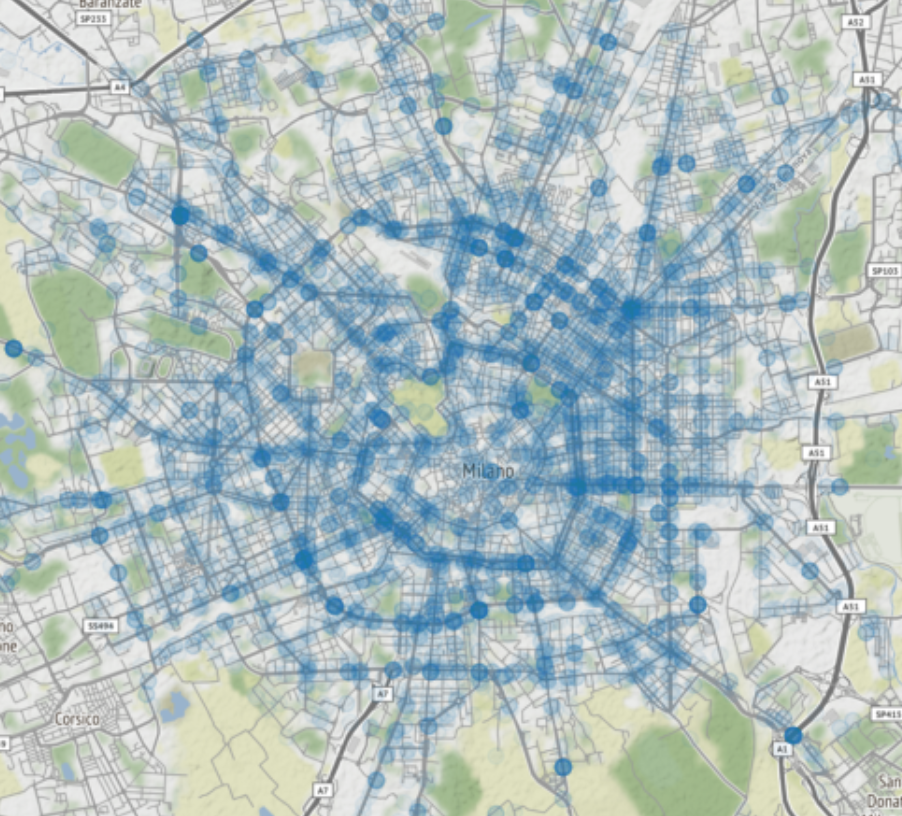
\includegraphics[width=\linewidth]{../src/incidenti/geo_incidenti.png}
    \caption{Distribuzione di incidenti a Milano}
    \label{fig:geo_incidenti}
\end{figure}

%...


\newpage
\section{Incidenti e Linee dei Trasporti Pubblici}

Il dataset dei tragitti dei trasporti pubblici copre molta pi\'u superficie rispetto a 
quello degli incidenti.
Dopo aver eliminato alcune linee di autobus che risultavano troppo in periferia, 
si nota comunque che i trasporti pubblici coprono la maggior parte di Milano.

\begin{figure}[!ht]
    \includegraphics[width=\linewidth]{../src/atm/mappa_2.png}
    \caption{Linee Autobus e Tram a Milano}
    \label{fig:geo_trasporti}
\end{figure}

Se a questi ultimi vengono sovrapposti i dati sugli incidenti, 
si pu\'o notare che la maggior parte dei luoghi con alta concentrazione di incidenti sono 
attraversati da linee di autobus. Nel caso di Corso Ventidue Marzo, si ha anche una linea di tram.
%...
\subsection{Il Pav\'e influisce sull'incidentalit\'a?} Spesso le linee di tram coincidono con
strade in pav\'e
%...
Servirebbe una mappa delle strade in pave a Milano..

% fine della subsection
Dalla sovrapposizione delle mappe, si pu\'o notare anche che, alcune strade con alta incidentalit\'a 
sono parallele a linee di autobus. Un esempio \'e quello di zona Navigli, 
dove le vie interessate sono:
Viale Gian Galeazzo e Viale Beatrice D'Este, parallele a Viale Col di Lana e Viale Bligny.
La stessa cosa si pu\'o notare su Viale Gabriele D'Annunzio e Viale Gorizia e Coni Zugna.

\begin{figure}[!ht]
    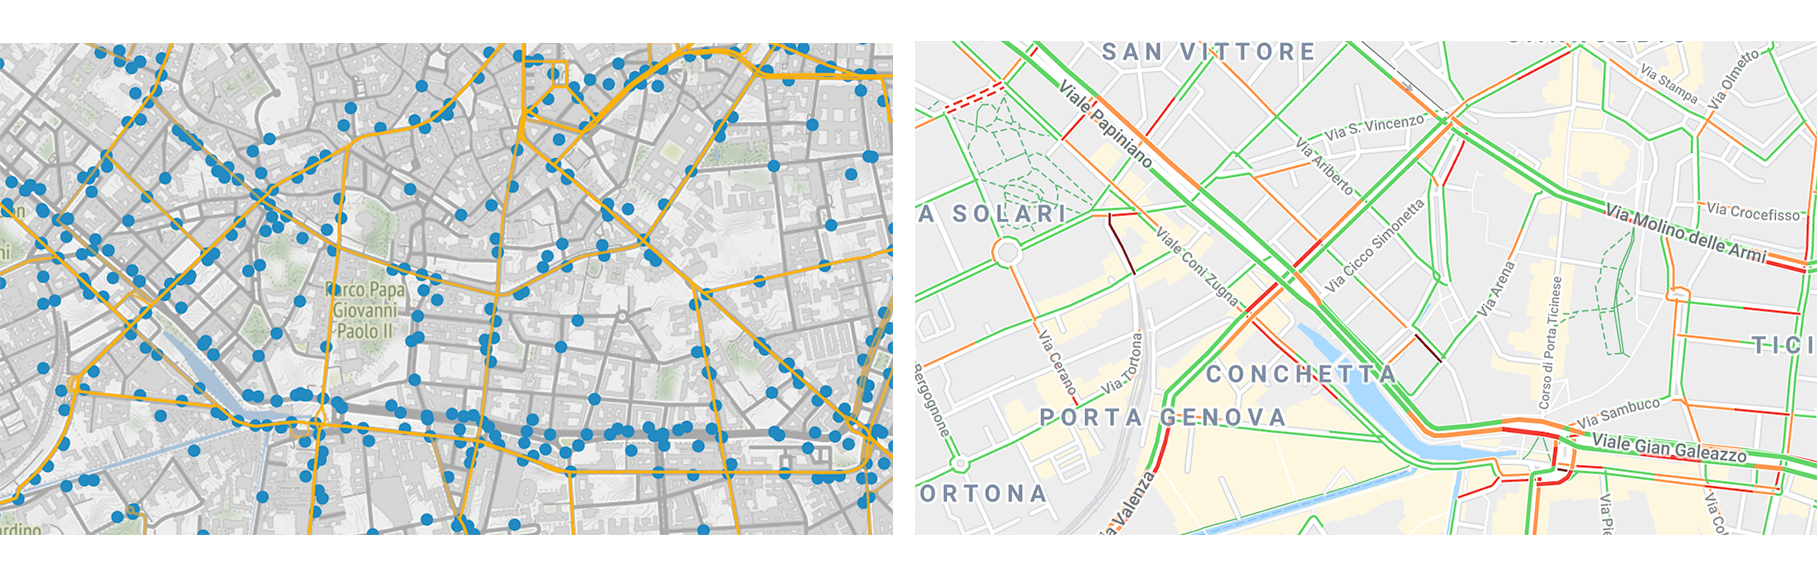
\includegraphics[width=\linewidth]{../src/atm/navigli.png}
    \caption{Linee Autobus e Tram a Milano}
    \label{fig:navigli}
\end{figure}

Anche vicino a corso Ventidue Marzo si pu\'o notare lo stesso fenomeno, 
tra Viale Bianca Maria e Viale Premuda.

\begin{figure}[!ht]
    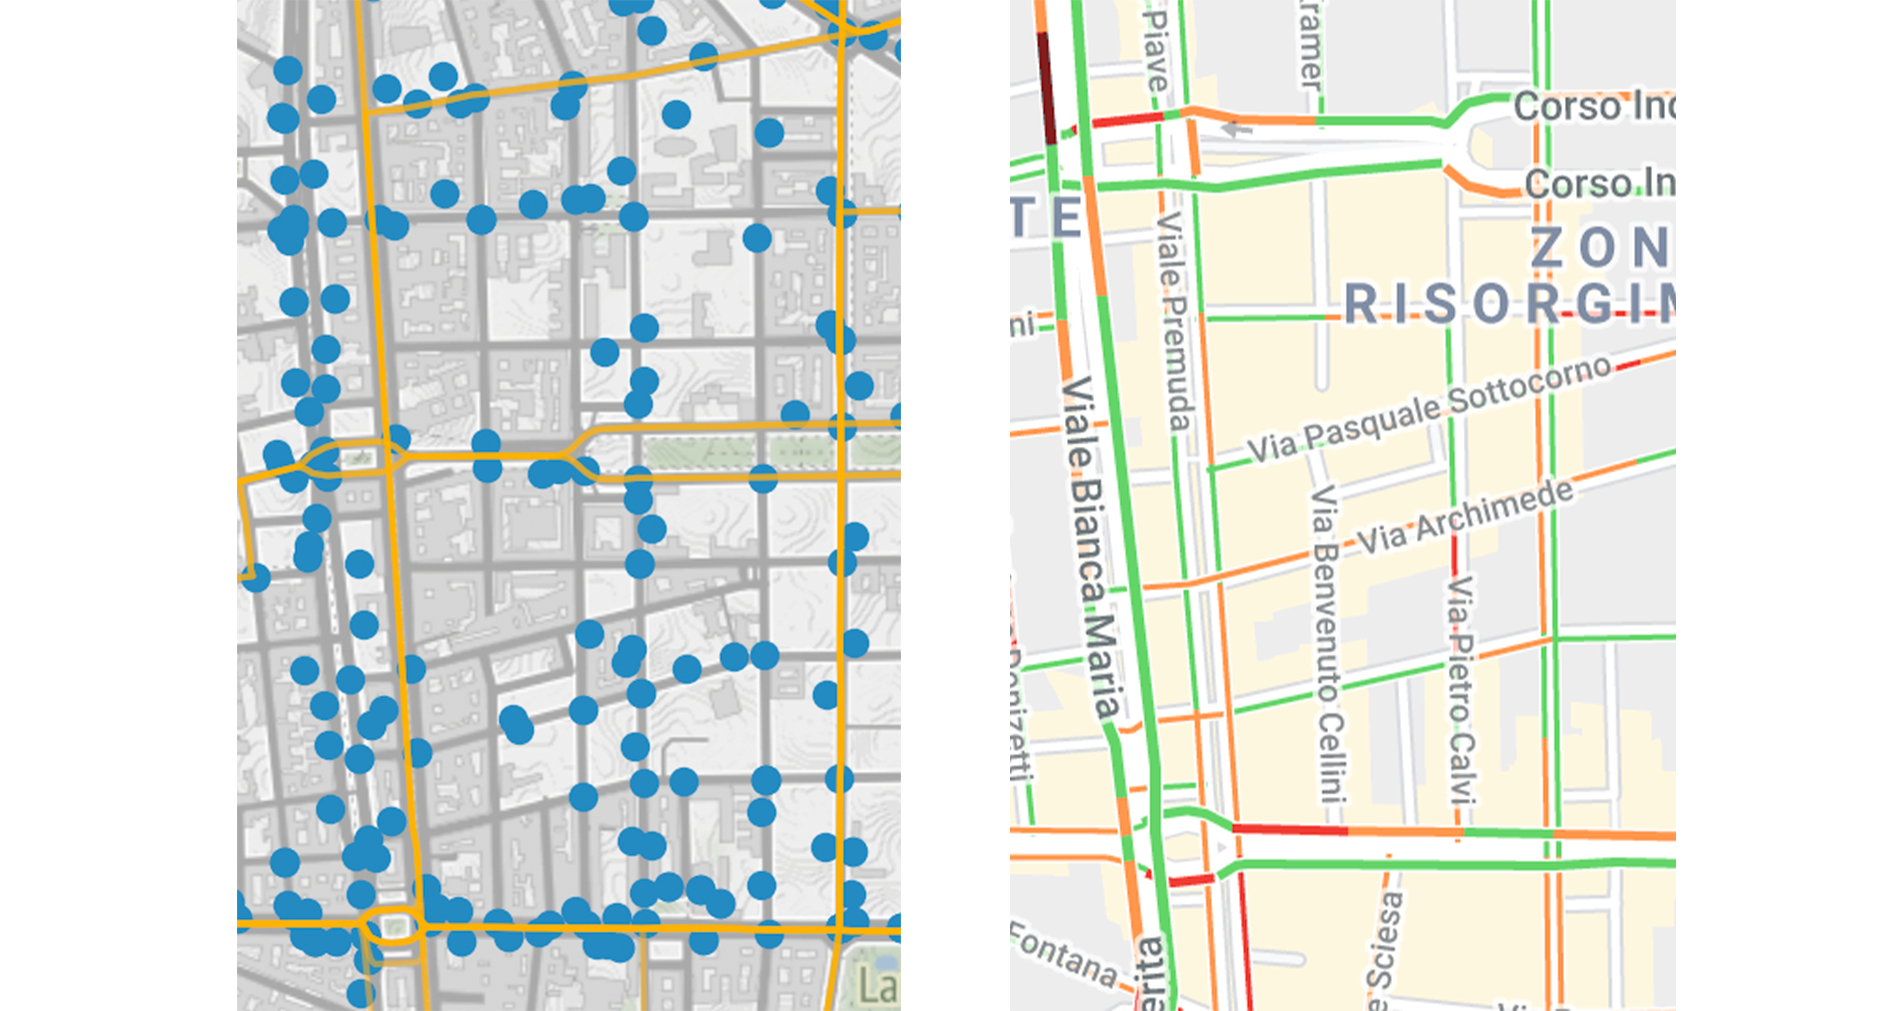
\includegraphics[width=\linewidth]{../src/atm/22_marzo.png}
    \caption{Linee Autobus e Tram a Milano}
    \label{fig:22_marzo}
\end{figure}

%...

\newpage
\section{Incidenti e Piste  Ciclabili}

\newpage
\section{Incidenti e Autovelox}

Per sapere se gli autovelox hanno influenza sull'incidentalit\'a, 
bisognerebbe innanzi tutto sapere quando sono stati posizionati i dispositivi, e solo a quel punto, 
avendo dati su incidenti prima e dopo l'installazione, sarebbe possibile trarre conclusioni.

Alcuni dati sull'installazione di autovelox esistono per l'anno 2014, tuttavia i dati 
riguardo agli incidenti sono solo riguardanti l'anno 2016, in quanto Istat non ha rilasciato 
le posizioni degli incidenti in altre annate.

%...


\newpage
\section{Incidenti e Meteo}

%%%%%%%%%%%%%%%%%%%%%%%%%%%%%%%%%%%%%%%%%%%%%%%%%%%%%%
\newpage
\chapter{Dati su Incidenti}

Per quanto riguarda dati generali su incidenti in Italia, sono disponibili due dataset molto ampi, 
il primo, rilasciato da Istat, contiene dati dal 2010 al 2018 che riguardano campi come data, ora, 
numero di persone a bordo, tipo di incrocio, tipo di veicolo, ecc..
Il secondo \'e invece messo a disposizione da Automobile Club D'Italia (ACI) che contiene dati simili, 
ma in pi\'u mette a disposizione il luogo dell'incidente, come autostrada o strada provinciale.

\newpage
\section{Dati Istat}


\newpage
\section{Dati ACI}

\newpage
\subsection{Quali sono le autostrade con pi\'u incidenti?}
\begin{figure}[!ht]
    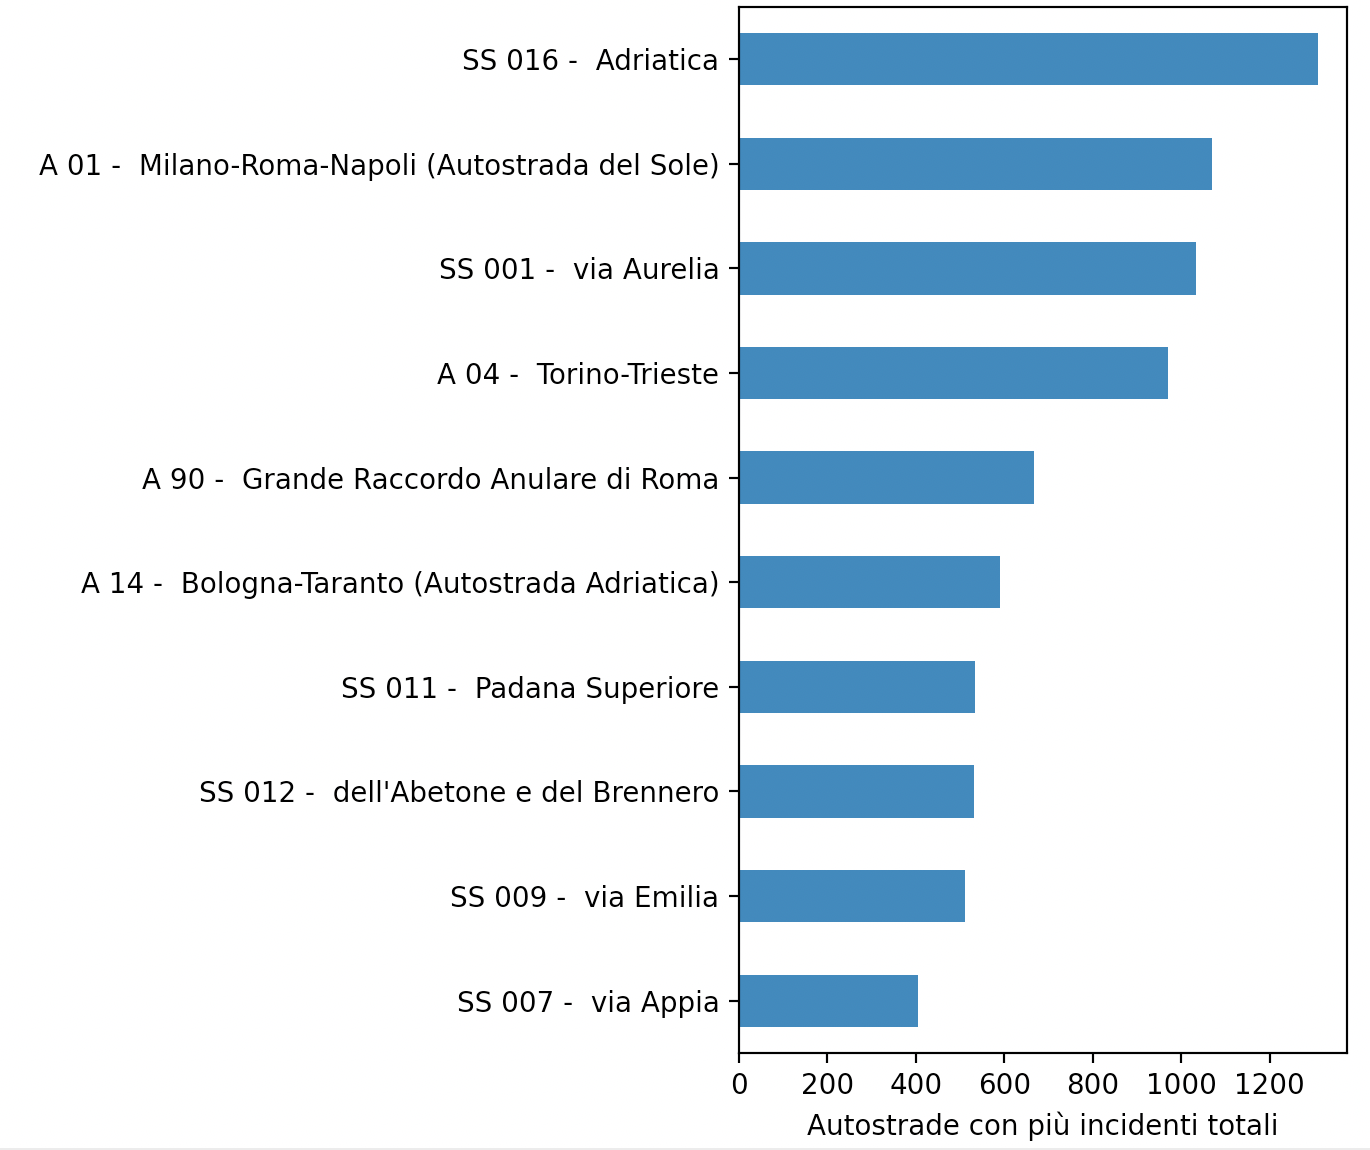
\includegraphics[width=\linewidth]{../src/incidenti/incidenti_aci/autostrade.png}
    \caption{Autostrade con pi\'u incidenti nel 2018}
    \label{fig:incidenti_autostrade}
\end{figure}

Si pu\'o notare subito che le autostrade con più incidenti sono anche quelle più trafficate, come 
l'Autostrada del Sole e l'Adriatica.


%...


\'E possibile anche capire quando questi incidenti avvengono, perch\'e ACI ha reso disponibili il mese 
dell'incidente.

\newpage
\subsection{In quali mesi avvengono pi\'u incidenti?}
\begin{figure}[!ht]
    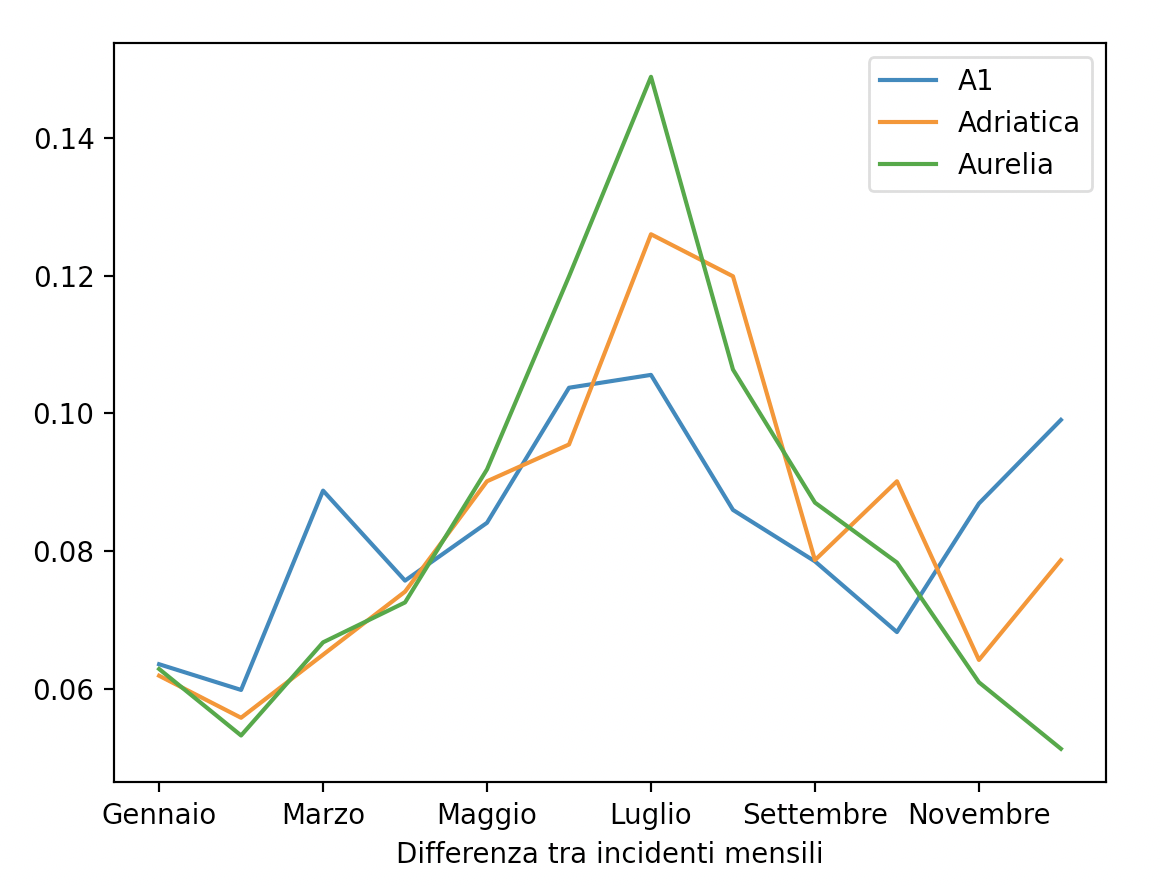
\includegraphics[width=\linewidth]{../src/incidenti/incidenti_aci/mesi_autostrade.png}
    \caption{Incidenti per mese nel 2018}
    \label{fig:incidenti_per_mese}
\end{figure}

Le curve sono state normalizzate per bilanciare il volume di incidenti maggiori per 
l'autostrada Adriatica.
L'Adriatica e l'Aurelia, autostrade utilizzate molto durante i mesi caldi, hanno un picco di 
incidenti in Luglio e Agosto, mentre l'A1, ha picco più basso in Agosto, probabilmente 
perchè bilanciato dagli incidenti in inverno intorno a Milano.

% controllare se avvengono più incidenti in inverno intorno a milano

%%%%%%%%%%%%%%%%%%%%%%%%%%%%%%%%%%%%%%%%%%%%%%%%%%%%%%
\newpage
\chapter{Dati su Meteo}

\bibliographystyle{plain}
\bibliography{Biblio}
%\addcontentsline{toc}{chapter}{Bibliografia}

\end{document}
